\chapter{Review of Related Literature} \label{sec:back}
Image vectorization has been a long and well-researched field. One of the earliest works on the field dates back to 1982 with the paper by Jimenez, J. and Navalon, J. Their works have been focused on vectorizing digital images from natural scenes \cite{somexperimentsvectorization}. The techniques they have used, such as contour following, have been adapted in later works. Later works have made significant progress over their work and made use of hardware advancements such as GPU utilization for computational tasks.

The primary goal of vectorization is to support multiple resolutions without any loss in the original data. Vectorization is suitable for the task. However, various methods have been proposed that do not involve vectorization. In this chapter, we will explore the previous works done for vectorization and making images support larger resolutions.

\section{Image Upscaling} \label{sec:image-upscaling}
Raster images are commonly used in representing images. Therefore, these types of images tend to be scaled to different resolutions. The process of scaling these types of images to higher resolutions is called \textit{image upscaling} \cite{hoshyari2018perceptiondriven}, and is the most common forms of having raster images support larger resolutions. Naively scaling images would result in images with empty pixels between the shifted pixels, producing a mostly empty image. Thus, the empty pixels are coloured based on their position from, and colour and intensity values of their neighbouring pixels. This process is called \textit{interpolation} \cite{resizingimages}. Traditional interpolation algorithms can be classified into two types: Non-adaptive techniques, and adaptive techniques. Each of these types have their own method of resizing images and would produce different results, which may fit in with different objectives of different users \cite{interpolationtechniquessurvey}. Most recent works uses artificial intelligence to construct a scaled image with as little image quality loss as possible. These works uses neural networks, specifically convolutional and adversarial neural networks, to produce photorealistic upscaled versions of images with little to no distinguishable loss of image quality \cite{aigigapixelstory}\cite{progressivesisr}\cite{sisrgan}.

\subsection{Non-Adaptive Techniques}
Non-adaptive interpolation techniques only scale images horizontally, vertically, or both, by a certain scaling factor, the amount in which the image will be scaled to. They do not assume anything about the underlying image data, except that it is band-limited \cite{depixelizingpixelart}. This makes them computationally cheap \cite{interpolationtechniquessurvey}, but also suffer from artifacts such as sharp edge blurring and ringing artifacts \cite{depixelizingpixelart}. Nevertheless, these non-adaptive image interpolation techniques have been widely used in the industry and is standard across different raster image editing programs, such as Adobe Photoshop and GIMP \cite{photoshopinterpolationmethods}\cite{gimpinterpolationmethods}. The common non-adaptive interpolation techniques used are:

\begin{itemize}
	\item Nearest Neighbour
	\item (Bi)linear Interpolation
	\item (Bi)cubic Interpolation
\end{itemize}

\subsubsection{Nearest Neighbour}
Nearest Neighbour is the simplest interpolation method to understand. At the high-level, nearest neighbour simply enlarges the size of each individual pixel by a certain factor.

At the lowest level, though this \textbf{may} differ implementation-wise, the algorithm will refer back to the original unscaled version to obtain the appropriate colours for each empty pixels in between the shifted pixels in the scaled image. Each empty pixel in the scaled version will map itself to a corresponding pixel in the original image. This is done by obtaining the square coordinates of the empty pixel and dividing the coordinates by the scaling factor. Note that the coordinate system in images starts its origin from the top left, instead of the bottom left. We may acquire a decimal as a result of dividing the coordinates, of which we will floor the values. The resulting coordinates can be mapped to a pixel in the original image. We will then use the mapped pixel's colour as the colour of the empty pixel we are calculating the colour for. The interpolated pixels can be seen as a set $I$, as quantified by the equation below.

$$ I = \{i | i = C((\lfloor\frac{e_{x}}{s}\rfloor, \lfloor\frac{e_{y}}{s}\rfloor))\}, s > 1, e \in E\ $$

$s$ is the scaling factor, $C$ is the function that gets the colour of a pixel based on its coordinate, and $E$ is the set of empty pixels that are in between the shifted pixels when naively upscaled. The resulting image will look blocky since the pixels are just enlarged. However, this will be ideal for pixel art \cite{resizingimages}.

\subsubsection{(Bi)linear and (Bi)cubic interpolation}\label{sec:bilinear-bicubic-interpolation}
Both of (bi)linear and (bi)cubic interpolations schemes are fairly similar to one another. The colours between the empty pixels between them are based on the values of the colours of the shifted pixels.

Each empty pixel acquire most of their colour from the nearest shifted pixel and least from the farthest shifted pixel. This process can be thought be thought of using graphs. In linear interpolation, the pixel colours can be viewed as the values of the y-axis, and the x-axis consists of the shifted pixels in the scaled image. The data points that are plotted are shifted pixels and are connected by a linear straight line. The colours of the empty pixels can then be computed by obtaining the y-value of the x-value of the pixel. Cubic interpolation is also the same process. However, the lines connecting the data points in the graph are cubic, i.e. smoother.

% Add more details on this part.

\subsection{Adaptive Techniques}
Image upsampling can also be performed with adaptive techniques. Adaptive techniques do not naively increase the increase the number of pixels with some approximate in a scaled image. Rather, they use the information of the raster image to fill up the now empty pixels when scaling images. The features they consider include intensity value, edge information, and texture \cite{interpolationtechniquessurvey}. However, the results may not be what is expected of.

\subsection{Super Resolution Methods}
Super resolution methods are processes of generating high-resolution images from low-resolution image input. Each method has different assumptions of the raster input and evaluation criteria. There are super resolution methods that target specific classes of input such as faces, scenes, and graphics artworks. Others are targeted towards generic input, in which the priors are based on image primitives such as edges and segments \cite{sisrbenchmark}.

\begin{figure}[h]
	\centering
	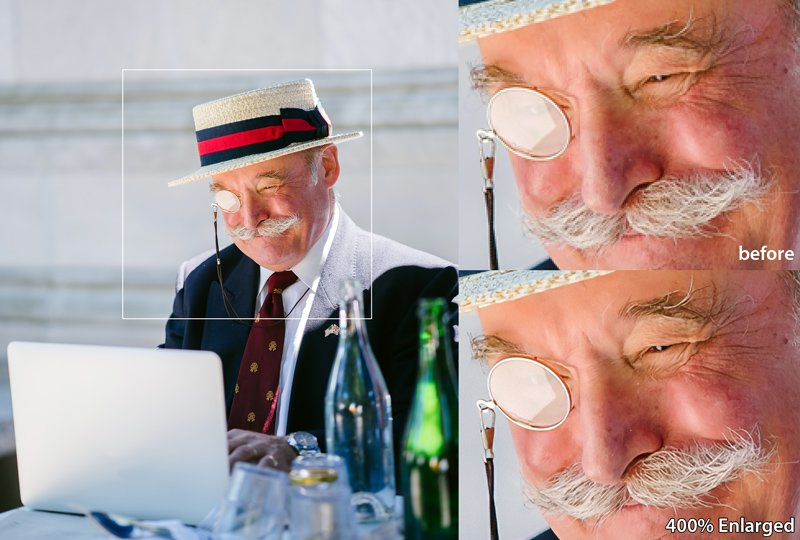
\includegraphics[scale=0.5]{images/chap02-rrl/aigigapixel-result.jpg}
	\caption{This a result of an raster image scaled to super resolution using A.I. Gigapixel. The left image is the original raster image. The top right is the normally scaled output. The bottom right is the output produced by A.I. Gigapixel. Image obtained from \protect\url{https://topazlabs.com/ai-gigapixel/}.}
	\label{fig:aigigapixel-result}
\end{figure}

Recent approaches to super resolution involves the use of artificial intelligence. One such approach is a commercial desktop application called A.I. Gigapixel by Topaz Labs. Images can be scaled by the A.I. Gigapixel with great accuracy. It uses neural networks and the computational power of the GPU to produce super-resolution results. It can also run on a laptop. However, it takes 20 minutes to run on a laptop, and a few minutes on a high-end GPU \cite{aigigapixelstory}. Another approach based on artificial intelligence and neural networks has also been proposed by Wang, Y., Perazzi, F., and McWilliams, B. In their work, they use a progressive approach to scale images to super resolution with the use of generative adversarial networks.

\section{Vectorization of Images}
Various methods have been proposed throughout the years in the pursuit of supporting larger resolution without any reduction in image quality through vectorization. Typically, vectorization methods target specific inputs, such as natural images or artist drawn images, as certain methods are unsuitable for different inputs. Hoshyari, S., et. al. states that vectorizations targeted at natural images frequently produce inconsistent results when applied to artist-drawn imagery such as logos, and simple graphic illustrations \cite{hoshyari2018perceptiondriven}. No matter what the methods used are, they produce vector graphics that will vary in quality, photorealism, and artistic look (view \cite{hierarchicaldiffusioncurves}, \cite{barendrecht2018locally}, and \cite{anovelmethodforvectorization} for a comparison of the results of various vectorization methods).

Despite vector graphics providing a compact and alternative form of representing \cite{realtimevectorizationgpu}, it is important to remember that due to the inherent characteristics of vector primitives where certain fine details of raster images cannot be accurately represented in vectorized form, vector images will only be giving approximations of the details of images \cite{optimizedgradientmeshes}. Nevertheless, finding the perfect balance for image level of detail and image vectorization is an endeavour that is left as an exercise for users \cite{anovelmethodforvectorization}.

Note that there are multiple possible vectorization outputs for a single raster image, with many outputs possibly being similar to one another and can be considered good enough for use. The \textit{locally} "best" vectorization of some raster input among those possible vectorizations is determined by the vectorization method utilized.

Image vectorization can be dated as far back as the early 1990s, though experiments have started since 1982 at the earliest \cite{somexperimentsvectorization}. Commercial packages, both proprietary and open source, have image vectorization tools whose quality vary. The packages include Adobe Illustrator (Live Trace), Corel CorelDRAW (PowerTRACE), and Inkscape (based on Potrace \cite{inkscapepotrace}) \cite{hoshyari2018perceptiondriven}. Their wide adoption, though impressive, do not always immediately translate to quality vectorizations. The current available methods still have their own shortfalls and are still in active development. As a result, manual vectorization are still being performed in many industries that heavily require vectorizations \cite{vectorizationoflinedrawingspolyvector}.

\subsection{Natural Images Vectorization}
Many raster images widely used today are photographs. They contain fine details and lush colour depth that are prominent in the real world. These photographs are also called natural images in digital image processing. Increasing their resolutions would entail using image upscaling techniques (see \ref{sec:image-upscaling}), especially the standard classical approaches. This would give the chance of producing low quality images \cite{depixelizingpixelart} when super resolution methods are not utilized. Vectorization of these natural images are then an alternative to producing high quality higher resolution images.

Vectorization methods targeted at natural images consist the large body of work that deals with automatic vectorization. The core method of these algorithms involves the reliance on edge detection and/or region segmentations to cluster large quantities of pixels together into larger regions \cite{depixelizingpixelart}. These regions are then filled with either a solid color \cite{anovelmethodforvectorization}, or gradients via gradient meshes \cite{optimizedgradientmeshes}\cite{barendrecht2018locally} or diffusion curves\cite{hierarchicaldiffusioncurves}.

\begin{figure}[h]
	\centering
	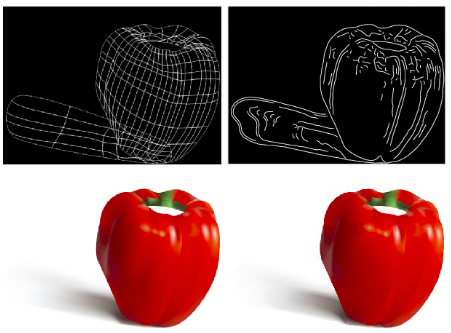
\includegraphics[scale=1.0]{images/chap02-rrl/diffusion-curves.png}
	\caption{The left side shows a result of using gradient meshes when vectorizing natural image. The right side uses diffusion curves (and fewer curves) to vectorize an image.}
	\label{fig:diffusion-curves}
\end{figure}

One relatively recent work for vectorizing natural images uses hierarchical diffusion curves. This work was proposed by Xie, G., Sun, X., Tong, X., and Nowrouzezahrai, D.. Diffusion curves are defined using "curve primitives with colors set on both sides of it". In simplified wording, a diffusion curve is a curve with colours diffusing away perpendicularly to the curve. Their work revolves around tracing the curves in a raster image in such a way that produces an accurate final vector output. The traced curves are only sparse. They are not restricted to natural images only as their method can be used in cartoon images as well. Their results are comparable to that of those that use gradient meshes. Observably, the results are impressive and matches the raster input. Their work, from their experiments, can take from a few seconds to 11 minutes, at the most. Note that they experimented on a PC with an 3.5 GHz Intel Core i7-3770K and an Nvidia Quadro 6000.

Another work that vectorizes natural image targets is that of Birdal, T., and Bala, E.. Their vectorization approach does not produce a near-accurate vectorization of the raster input. Rather, their vectorization produces a flat art style output. Their approach uses segmentation to identify regions. The authors offer three different segmentation methods, all having an impact on the final vectorization output:

\begin{enumerate}
	\item \textbf{Statistical Region Merging} (SRM) considers the image as an unknown scene. Colours are sampled in this method from a set of distributions that represent image pixels. To summarize, the pixels are segmented based on the observed mean values of the pixels.
	
	\item \textbf{Colour Structure Coding} (CSC) is a technique that is hierarchical and region-growing that consists of two phases that essentially groups pixels of similar colours together. The colour similarity is determined as similar when the Euclidean distance of two colours is smaller than a certain threshold.
	
	\item \textbf{Graph-based Segmentation} is another approach that can be used and is similar to SRM. In their work, they used a segmentation technique proposed by Felzenszwalb, P., and Huttenlocher, D. \cite{efficientgraphbasedimagesegmentation}.
\end{enumerate}

Boundaries are then extracted from the segmentation outputs. The boundaries are then fitted with a spline. In their work, they used cubic Bezier curves to represent the vectorizations of those edges. The final final vector curves, which will now form shapes when connected, are filled with the approximation of the colour of the region in the raster image enclosed by the region \cite{anovelmethodforvectorization}.

Video is just a series of natural images. As such, it can be a target for vectorization. The work of Xiong, X., Feng, J., and Zhou, B. deals with vectorization of video. They are not vectorizing video as a post-processing step. Rather, they are vectorizing video in real time. They made it possible through the use of GPUs. Graphics processing units (GPUs, for short) have been in use to accelerate processing of tasks. Their parallelized nature, since they consist of small, efficient cores that handle multiple tasks that run in parallel, allow for faster computations \cite{gpuacceleratedcomputing}. In vectorizing video in real time, they first detect the boundary pixels of each line. These boundary pixels are pixels that determine the start and end of some region in a line. This stage essentially segments the current video frame. This process is done via a scanline approach. Due to the relative independence of each line during this stage, parallelism can be utilized to reduce the amount of time needed to perform this stage. Pre-countouring is then performed to identify the relationship of the regions in a line to the regions in adjacent lines. This is done to identify how regions in one line is connected to larger region in the video frame. This stage is also parallelized since the relationship is identified only being determined between two lines at a time. Pre-contouring will now lead to contouring which identifies the different regions in a video frame. The edges of each region is computed a loop from which a vectorization is will be performed upon. This is done with the CPU due to the frequency of memory access necessitated by this step. The loops are then simplified and vectorized with a set of line segments through a process similar to that of Active Countour Modelling, where each loop is processed with a divide-and-conquer strategy. The independence of each loop from one another allows for this step to be highly parallelized. Their experimentation shows that they were able to vectorize videos with an average video frame rate of 48 fps, and vectorize a 2500x1800 resolution typed page in just 40 ms. They have performed their experimentation using CUDA with a PC that has a 2.5 GHz quad-core CPU (brand unspecified), 2.75 GB RAM, and an Nvidia GeForce GTX 260+ \cite{realtimevectorizationgpu}. Their work is a demonstration that GPU utilization for parallel execution is beneficial to speeding up vectorization. However, due to their use of line segments as the vector primitive for their work (unlike other works such as those of Kopf, J., and Lischinski, D. \cite{depixelizingpixelart}, and Xie, G., Sun, X., Tong, X., and Nowrouzezahrai, D. \cite{hierarchicaldiffusioncurves}), the result may not be what is expected of the final vectorization.

\subsection{Vectorization of Semi-Structured Images and Artworks}
Artwork, especially its subset, semi-structured images, is undeniably widely used around the globe. They are used to convey information, and express ideas. Both purposes would infer the necessity to maintain the high, or at least good enough quality images of those artworks to properly fulfill their tasks. Vectorization of these images would ensure that the quality of the image is kept at any resolution possible without any degradation. In the pursuit for quality vectorizations, many papers have been proposed that target specific inputs (such as pixel art, or small resolution images) and give out varying vectorization results.

A framework that optimizes bezigons, closed paths composed of Bezier curves, to match their raster counterparts as much as possible was proposed by Yang, M., et. al. as a vectorization process. Their work takes bezigons as input, of which they obtain either using pre-existing vectorization methods or extracting them from the raster image by segmenting the image into a set of regions then fitting piecewise Bezier curves on the region boundaries. The input is called the \textit{initial bezigons}. These initial bezigons are then optimized to reflect the raster image as close as possible. In optimizing the bezigons, they use a non-linear optimization algorithm (to be referred as *NLOAs* from hereafter) such as NEWUOA and conjugate gradient. Being an optimization-centered process, their process requires a method to evaluate their optimizations. Evaluating the vectorization output would involve getting the rasterization of the output and comparing it with the original raster image. Since there are various rasterization functions, a good enough rasterization function that works well with NLOAs is required. Using discontinuous and piecewise rasterization functions yields poor results during optimization. As such, a continuous rasterization function is required. Yang, M., et. al. chose to use a rasterization approach that utilizes a hierarchical Haar wavelet representation. The key component, which we view as a primary contribution of their work, is the energy $E$ used to evaluate the vectorized outputs. $E$ is the sum two parts: (a) the data energy, and (b) the prior energy. The data energy refers to the distance of the input raster image and the rasterization of the vectorization output. The prior energy refers to the severity of unreasonable bezigons. These bezigons would typically fall under one of the following categories, as per the work's authors intensive experimentation: (a) self-intersection, (b) false corners with small angle variations, (c) short handles, and (d) twisted sections. A larger $E$ would indicate a more inaccurate vectorized output. As such, optimization of bezigons, as it is their work, would be to minimize $E$. Basing from their experiments, they produce high quality vectorizations that are superior to the results of Vector Magic and Adobe LiveTrace. However, the frameworks yields poor results when vectorizing noisy or low-resolution inputs. Assuming that the experimental results be any sign for the actual theoretical speed, the execution time of this ranges from 10 seconds to 10 minutes, depending on the complexity of the shapes being vectorized. It is important to note that their implementation is not optimal and is written in Python, which provides a significant overhead. An implementation in a static, compiled language is expected to yield faster optimization speeds \cite{effectiveclipartimagevectorization}. Basing from personal experience in hand vectorization, this framework resembles manual vectorization in that a bezigon is initially created that does not immediately match the raster image. The bezigon is later adjusted to fit the raster image boundaries. Being that they have proposed a framework, their work can be viewed as an optional and/or complimentary post-processing step to tweak pre-vectorized accuracy-ambiguous images, rather than a complete alternative or replacement of pre-existing and well-established vectorization methods, such as Adobe LiveTrace, and Potrace. At least one work, specifically that of Hoshyari, S., et. al., has already stated that their work is complimentary to this \cite{hoshyari2018perceptiondriven}. The only disadvantage to this framework is that it requires multiple iterations before settling on an optimal vector solution, which, consequentially, require some time to complete. It is also unclear whether the framework becomes more computationally expensive as the raster image size becomes larger as their paper does not indicate whether it is so or not.

Another form of digital art that is a target of vectorization is pixel art. Pixel art is a form of art where the level of detail is limited to the pixel level. This type of art tends to be blocky, and is reminisce of the art style of retro-era games. The work of Kopf. J, and Lischinski, D. specifically targets pixel art. As with other vectorization methods, their work detects edges of which they fit curves to create a final vector result. Due to the inherent property of pixel art, their work is met with a few non-trivial challenges. The authors have identified four:

\begin{enumerate}
    \item Every pixel matters, since a pixel can possibly represent a different feature given its colour is different enough from its neighbours, Additionally, each pixel can be viewed as an approximation of certain details in the overall image.

    \item Pixels in a pixel art look connected at original scale, but disconnected when magnified.

    \item The reduced level of detail in pixel art gives way to locally ambiguous configurations, in which it is unclear which pixels are part of which features.

    \item Lastly, jaggies, collection of pixels that we perceive as forming jagged lines, in pixel art make differentiate features from pixelization artifacts hard.
\end{enumerate}

The proposed vectorization method of Kopf, J., and Lischinski, D. would first involve creating a similarity graph that would connect similar pixels with one another via edges. In this case, similar pixels would refer to pixels with similar colours. It should be noted that their work has some basis on Gestalt psychology in order to closely reflect what a human will imagine the final vector output to be. In integrating Gestalt psychology, they utilized heuristics to help identify which nodes in the similarity graph are to be connected or not. Once a similarity graph has been constructed, a Voronoi diagram, which consists of Voronoi cells, is made based on the similarity graph. The diagram now represents a rough shape of the object. The connected visible edges of the diagram, simplifyingly, are converted into quadratic B-spline curves. Related to the work done by Yang, M., et. al., optimization of the resulting quadratic B-spline curves are performed. Optimization involves the "minimization of a sum of per-energy nodes". A node, in this context, refers to a single endpoint of a curve. The energy $E$ of each node $i$ is computed to be the sum of both smoothness and positional terms, $E_{s}^{(i)}$, and $E_{p}^{(i)}$, respectively.

$$ E^{(i)} = E_{s}^{(i)} + E_{p}^{(i)} $$

The smoothness term, $E_{s}^{(i)}$, measures the absence of curvature in the curve region influenced by node $i$. On the other hand, the positional term, $E_{p}^{(i)}$, measures the distance a control point node has moved away from their initial positions. The latter term is a prerequisite to prevent objects from changing too often. The control points are allowed to move freely within a relatively small region around their origin location, but are penalized when they deviate too far away. Not all nodes are optimized as a random walk is performed per iteration do identify which nodes will be optimized. The resulting vector image, after optimization, may have nodes that were not constrained. As such, these unconstrained nodes are computed a new location using harmonic maps. This tweaking results in distortion of cells in the Voronoi diagram. Additionally, corners in the pixel art are detected via heuristics to make sure these corners are given sharp lines, rather than a smooth curve. This work has yielded excellent results that closely resembles that of the original pixel art image. Comparing this with the results of previous works for vectorization, especially those with an inclination towards pixel art, this work has produced results that are comparable or superior (for example, when comparing against Adobe LiveTrace). The published execution time of the work opens it up for the possibility of use in vectorizating videos of retro games, especially when done in real time. The work, however, is limited hand drawn pixel art. Downsampled pixel art tend to look anti-aliased, which makes these inputs closer to natural images --- inputs this work was not designed for. The results produced by this work will not always agree with human perception \cite{depixelizingpixelart}. When viewed at a naive resolution independency angle, it would seem that this work is a step in the wrong direction as a simple nearest neighbour scaling algorithm can be applied to pixel art to support higher resolutions, as the algorithm is compatible with this type of input. However, when looked from a far enough distance, pixel art is viewed to be smooth and continuous. Simply upscaling such images would have it retain its blocky nature. This work by Kopf, J. and Lischinski, D. offers a way to vectorize pixel art to \textbf{not only} support higher resolutions, but as well as providing a \textit{smoother}, not blocky, output that closely matches the perception of the figure.

Humans naturally have an expectation of the vectorization output of a certain image. Hoshyari, S., et. al. proposed a vectorization method that exploits human perception to produce accurate vectorizations of images. Their work is primarily driven by Gestalt psychology in the attempts to create a vectorization that is close to human expectations. The authors have identified four principles that they integrated with their work:

\begin{enumerate}
	\item \textbf{Accuracy}, which states that we expect the rasterization of the vector output to be the same pixelized content as the original raster image.

    \item \textbf{Continuity}, which states that despite the blocky nature of pixel art, they are perceived as a smooth line or curve and not necessarily full of corners.

    \item \textbf{Simplicity}, which states that viewers have a preference for simpler geometric interpretations of the raster image.

    \item \textbf{Closure}, which, aside from being a part of human breakups (sometimes not at all), states that human observers would mentally segment objects at points, with a negative curvature minima, with a pair point opposite of them with a negative minima.
\end{enumerate}

Unlike previous vectorization methods, this work utilizes machine learning in one stage of the work to help generate vectorizations. Machine learning is used for detecting corners in a raster image. Corner detection is essentially to allow for accurate vectorizations especially at, well, corners. In the work, they have used random forests, trained through supervised learning with a training/validation data set of 158 raster images (with the training images being 8/16/32/64/128/256 pixels on each size), to detect corners. In their experiments, random forest classifiers have produce more accurate corner detections than neural networks. After corner detection, they would obtain an initial set of possible corners and an initial vectorization performed with the use of a version of the fitting algorithm proposed by Baran, et. al. \cite{sketchingclothoidsplines}. This set is expected to possibly contain corners that do not match with human perception. As such, an iterative corner removal process is employed to prune away corners that do not match with human expectations. In this stage, each corner is systematically removed to evaluate if it is a corner that aligns with human perception in accordance with the four aforementioned principles. It is removed if the resulting vectorization produced without it is better than the one with it. The iterative corner removal process completes once all corners have been evaluated. The final vectorization is then regularized. Regularization involves locating characteristically similar, but not identical, splines and primitives and enforcing them to be identical. These located primitives and splines are adjusted to have the same characteristics. This process produces a simplified vectorization output, in line with the simplicity principle utilized in the work. According to their experimental results, their results are superior to Adobe LiveTrace, Vector Magic, and Potrace. Observers preferred their results than those generated by the aforementioned vectorization methods. They also find the results on par with manually produced vectorizations. Despite the results, however, their work becomes computationally expensive as the input size becomes larger. Additionally, their work is designed only to vectorizing clean quantized images. Anti-aliased and noisy inputs will likely generate unexpected final vectorization result. Filtering to quantize those types of inputs would produce artifacts that would impact the vector result. Future work includes addressing these issues \cite{hoshyari2018perceptiondriven}. The proposed corner detection stage in this work can be improved, possibly by using a different neural network or classification method, to reduce the necessity to use an iterative corner removal process and may be used as a necessary step in future vectorization methods. The emphasis on the utilization of Gestalt psychology principles to produce results near to human expectation is also a component that must be given note and should be considered by future works.

% Place items into separate lines, for the sake of the reader and readability, and to take up more pages.

% Talk about other works.